% Define roman numerals for front matter
\makeatletter\newcommand*{\rom}[1]{\Ifstr{#1}{0}{0}{\expandafter\@slowromancap\romannumeral #1@}}\makeatother

% Half title page
\thispagestyle{empty}
\null\vspace{4cm}
\begin{raggedleft}
    {\fontsize{24pt}{0pt}\selectfont \textbf{A Complete Introduction To Abstract Algebra}}\\
\end{raggedleft}

% Title page
\begin{titlepage}
    \null\vspace{4cm}
    \begin{raggedleft}
        {\fontsize{20pt}{0pt}\selectfont \textbf{A Complete}\\\textbf{Introduction To}}\\

        \vspace{0.4cm}
        {\fontsize{48pt}{0pt}\selectfont \textbf{ABSTRACT}}\\
        \vspace{0.15cm}
        {\fontsize{48pt}{0pt}\selectfont \textbf{ALGEBRA}}\\

        \vspace{0.5cm}
        {\fontsize{16pt}{0pt}\selectfont Version \version}\\
        
        \vspace{1.25cm}
        {\fontsize{20pt}{0pt}\selectfont Kan Onn Kit}\\
    \end{raggedleft}
    \vspace*{\fill}
\end{titlepage}

\newpage{}

% Edition notice
\clearpage\null\vfill
\thispagestyle{empty}
\begin{minipage}[b]{0.9\textwidth}
    \footnotesize\raggedright
    \setlength{\parskip}{0.5\baselineskip}

    Published by Kan Onn Kit\\
    Singapore
    \vspace{5cm}

    \textbf{A Complete Introduction To Abstract Algebra}\par
    Version \version
    \vspace{0.3cm}

    Copyright \copyright \ 2022 -- \the\year\ by Kan Onn Kit\par
    This work is licensed under a
    Creative Commons Attribution-NonCommercial-ShareAlike 4.0 International Licence.\par
    \pdfteximg{2.5cm}{images/CC_BY-NC-SA_4.0.pdf_tex}\\
    The full licence text is available at \url{http://creativecommons.org/licenses/by-nc-sa/4.0/}.\par    
    The source files for the project are available at \url{https://github.com/PhotonicGluon/Abstract-Algebra-Book}.
    \vspace{0.3cm}

    Typeset in 10pt \TeX~Gyre Pagella using PDF\LaTeX.
\end{minipage}

\vspace*{2\baselineskip}
\cleardoublepage

% "Quote" page
\thispagestyle{empty}
\vspace*{2cm}

\begin{center}
    \Large{\parbox{10cm}{
        \begin{raggedright}
            \Large
            Symmetry is a vast subject, significant in art and nature. Mathematics lies at its root, and it would be hard to find a better one on which to demonstrate the working of the mathematical intellect.
            \vspace{0.3cm}
            
            \hfill
            --- Hermann Weyl, 1952\\
            \vspace{-0.25cm}
            
            \hfill
            \normalsize
            ({\cite[p.~145]{weyl_1952}})
        \end{raggedright}
    }
}
\end{center}

\newpage

% Table of contents
\createtoc

% Acknowledgements
\chapter{Acknowledgements}
Undertaking such a monumental project is new to me, and I am indebted to the people who accompanied me on this journey.

I am eternally grateful to my parents, who have spent countless hours and an ungodly amount of effort to raise me into who I am today. Their omnipresent kindness, patience, and love for me are something I certainly do not deserve, and I thank them for taking care of me.

I would like to thank my tutor Leong Chong Ming, who got me interested in abstract algebra in the first place. His enthusiasm and eagerness to share his knowledge on the subject is the driving force behind my decision to write these books.

I am grateful for the help of my friend Low Ji Yuan, who has assisted me with countless revisions of the content in these books and given me another pair of eyes in the vetting of content.

I also sincerely appreciate the support from my mathematics tutors, Loke Weng Heng, Siow Yun Jie, and Teng Yen Ping, who have been there through my junior college years inspiring me with the wonders of mathematics. I am indebted to them for allowing me to excel in my final examinations.

My close friends, Aidan Tay, Gabriel Fong, and Low Ji Yuan, accompanied me through two years of schooling (and math jokes). I offer infinite thanks to them for sticking with me and for encouraging this math nerd to pursue his wacky projects.

A thousand thanks go out to my teachers at the School of Science and Technology, Singapore, and specifically my form teacher Lee Tsi Yew Samuel, who instilled important character values into me so I can excel in my future endeavours.

% Preface
\chapter{Preface}
Although algebra has a long history, it has undergone quite striking changes in the past few decades. Abstract (or modern) algebra is widely recognised as an essential element of higher mathematical education. However, the results that it showcases are often hard to grasp and understand without prerequisite knowledge or a heavy background in mathematics. Most books on this subject are crafted for undergraduates at universities. They are not for a general mathematics enthusiast or one who seeks to understand more about the inner structure of algebra that mathematicians encounter frequently.

The exploration of such structures is fundamental to the current underpinning of scientific inquiries. For example, groups are important as they describe the symmetries which the laws of physics seem to obey. Finite fields are also used in coding theory and combinatorics. I hope this series of books will inspire more people to learn more about abstract algebra, beyond the simple introduction presented here.

In addition, I find that, in most textbooks, important details are left for the reader to figure out independently, without providing any additional guidance or help along the way. Exercises and problems are provided for topics taught in abstract algebra, but only a handful have written solutions provided, leaving readers unsure of the correctness of their answers. I believe that the completeness of a textbook is essential; no claim made should be without justification (unless absolutely necessary). These books offer a more complete picture of abstract algebra by providing full-worked solutions to all exercises and problems posed.

This series of books serves to achieve several goals.
\begin{itemize}
    \item Provide a step-by-step explanation of core results from abstract algebra, without ambiguity of the results discussed.
    \item Demystify the core steps that many textbooks gloss over when proving results or when writing the solutions to problems/exercises.
    \item Ensure that results from abstract algebra are as accessible, as approachable, and as understandable for as many people as possible.
\end{itemize}
I hope that these books can accomplish these goals and let readers enjoy the wonders of abstract algebra.

\hfill{\textit{24 September, 2023}}

% Suggestions on the use of this book
\chapter{Suggestions on the Use of This Book}
\section*{General Information}
\begin{itemize}
    \item We include both exercises and problems.
    \begin{itemize}
        \item An exercise can be thought of as a simple ``self-review'' question. Exercises ensure that the content of a particular section is understood and should not be too hard to answer.
        \item A problem is a more holistic version of an exercise. Generally, solutions to problems require a thorough understanding of the current chapter and may require results from other chapters.
    \end{itemize}
    \item A consistent labelling system for all the results within and between parts is necessary for a project as long as this one.
    \begin{itemize}
        \item All definitions, axioms, examples, lemmas, theorems, propositions, and corollaries are consecutively numbered, using the format
        \begin{quote}
            \code{[CHAPTER].[SECTION].[NUMBER]}
        \end{quote}
        For example, the fourth statement in chapter 2, section 3 is labelled \textbf{2.3.4}.
        \item Exercises and problems are also numbered consecutively, using the format
        \begin{quote}
            \code{[CHAPTER].[NUMBER]}
        \end{quote}
        For example, the third exercise in chapter 2 is labelled \textbf{2.3}. Likewise, the fourth exercise in chapter 3 is labelled \textbf{3.4}.
    \end{itemize}
    \item The symbol ``$\qedsymbol$'' marks the end of a proof.
\end{itemize}

\section*{Chapter Interdependence}
The diagram on the next page shows chapter interdependence. It should be used in conjunction with the table of contents and notes listed.

\newpage
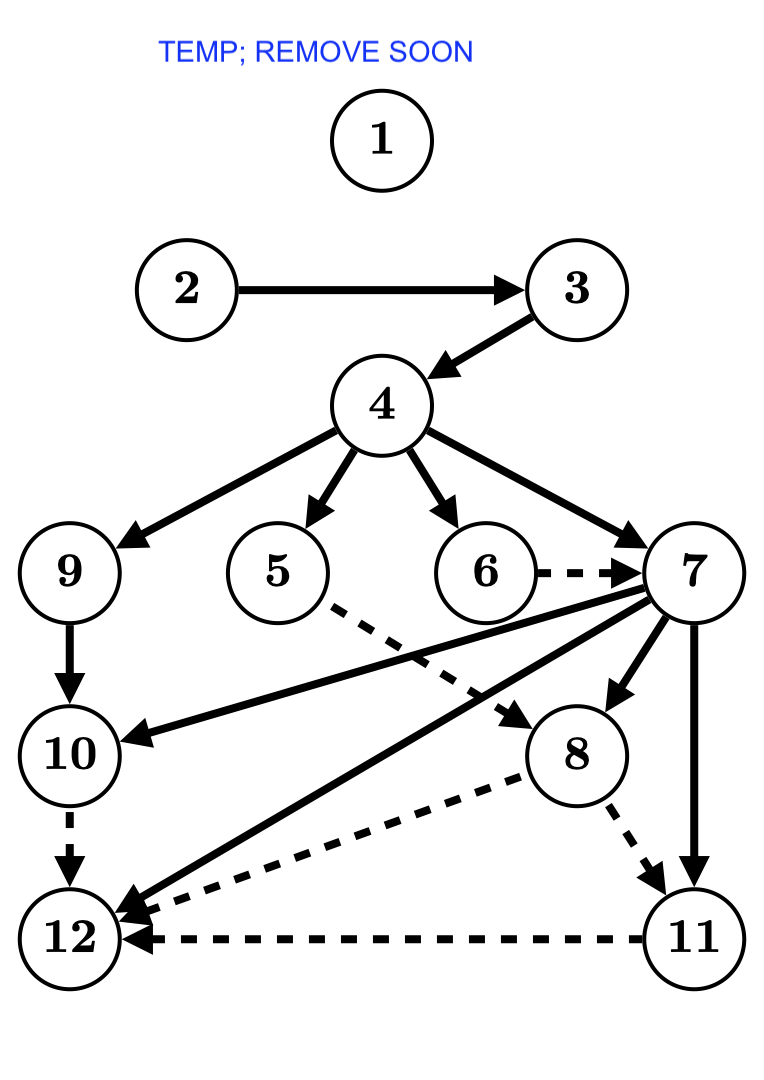
\includegraphics[width=\linewidth]{interdependence.png}

\newpage

\textbf{Notes}:
TODO: ADD
